\documentclass[bibliography=totoc,12pt,a4paper]{scrartcl}
\usepackage{amsmath, amssymb, amsthm}
\usepackage{enumerate}% schicke Nummerierung
\usepackage{graphicx}
\usepackage[english, ngerman]{babel}
\usepackage[T1]{fontenc}
\usepackage{lmodern}
\usepackage[utf8]{inputenc}
\usepackage{bigdelim}
\usepackage{multirow}
\usepackage{dsfont}
\usepackage[colorlinks=true,linkcolor=black, citecolor=black]{hyperref}
\usepackage{cite}
\usepackage[nottoc]{tocbibind}
\usepackage{empheq}
\usepackage{fancyhdr}
\usepackage{geometry}
\usepackage{lipsum}
\usepackage{tikz,pgfplots}
\usepackage{nicefrac}
\usepackage{graphicx}
\usepackage{subcaption}
\usetikzlibrary{shapes.misc}
\usetikzlibrary{matrix}
\geometry{a4paper,left=40mm,right=30mm, top=5cm, bottom=5cm} 

\def\@biblabel#1{\textcolor{red}{[#1]}}

\newtheoremstyle{linebreak}   % name
{3pt}                         % Space above
{3pt}                         % Space below
{}                            % Body font
{}                            % Indent amount 1
{\bfseries}                   % Theorem head font
{\newline}                    % Punctuation after theorem head
{.5em}                        % Space after theorem head 2
{}                            % Theorem head spec (can be left empty, meaning ‘normal’)
%\theoremstyle{linebreak}
\newtheoremstyle{exampstyle}
  {\topsep} % Space above
  {\topsep} % Space below
  {} % Body font
  {} % Indent amount
  {\bfseries} % Theorem head font
  {.} % Punctuation after theorem head
  {.5em} % Space after theorem head
  {} % Theorem head spec (can be left empty, meaning `normal')
\theoremstyle{exampstyle}
\newtheorem{defi}{Definition}%[chapter]
\newtheorem{satz}[defi]{Satz}
\newtheorem{theorem}[defi]{Theorem}
\newtheorem{propo}[defi]{Proposition}
\newtheorem{lemma}[defi]{Lemma}
\newtheorem{cor}[defi]{Korollar}
\newtheorem{bem}[defi]{Bemerkung}
\newtheorem{bsp}[defi]{Beispiel}
\newtheorem{folg}[defi]{Folgerung}
%bemerkungen oder Fließtext???
\numberwithin{equation}{section} 
 \newcommand{\newln}{\\&\quad\quad{}}
 \setlength\parindent{0pt}

\renewenvironment{abstract}
 {\small
  \begin{center}
  \bfseries \abstractname\vspace{-.5em}\vspace{0pt}
  \end{center}
  \list{}{%
    \setlength{\leftmargin}{12mm}% <---------- CHANGE HERE
    \setlength{\rightmargin}{\leftmargin}%
  }%
  \item\relax}
 {\endlist}


\usepackage{listings}
\usepackage{color}
 
\definecolor{codegreen}{rgb}{0,0.6,0}
\definecolor{codegray}{rgb}{0.5,0.5,0.5}
\definecolor{codepurple}{rgb}{0.58,0,0.82}
\definecolor{backcolour}{rgb}{0.95,0.95,0.92}
 
\lstdefinestyle{mystyle}{
    backgroundcolor=\color{backcolour},   
    commentstyle=\color{codegreen},
    keywordstyle=\color{magenta},
    numberstyle=\tiny\color{codegray},
    stringstyle=\color{codepurple},
    basicstyle=\footnotesize,
    breakatwhitespace=false,         
    breaklines=true,                 
    captionpos=b,                    
    keepspaces=true,                 
    numbers=left,                    
    numbersep=5pt,                  
    showspaces=false,                
    showstringspaces=false,
    showtabs=false,                  
    tabsize=2
}
 
\lstset{style=mystyle}

\begin{document}

\title{Quasi-Newton Methoden in der Formoptimierung}

\author{Daniel Luft \\ Prof. Dr. V. Schulz}

  \pagestyle{empty}

  % Ab sofort Seitenzahlen in der Kopfzeile anzeigen
  \pagestyle{headings}
  
\selectlanguage{ngerman}

\section{Resultate}
\subsection{???}

\colorbox{red}{l-bfgs springt schnell nahe Lösung: Verwandtschaft zu CG (nocedal + das paper zu konvergenz}
\colorbox{red}{erwähne, dass Gitter Probleme macht; eigentlich Neustart mit Gitter nötig; oder Lameparameter mit Funktion tweaken}
\colorbox{red}{wenn konvergiert, so vllt auch mit lokalen Minima...}
\colorbox{red}{Gitterunabhängig? Ordnung der Bilinearform mit der des Hesseoperators in übereinstimmung? Ausblick biharmonic?}
\colorbox{red}{plotte l-BFGs vs Gradient}
\colorbox{red}{mache Langzeit rechnung mit und ohne Line-search bei Pertubation}
\colorbox{red}{Programme als Wort, Rechtschreibfehler in anderen Chaptern}
\colorbox{red}{ eventuell bei Zeit die Hintergrundeinstellung bei Paraview bei allen Bildern gleich machen, sprich jedes mal X-Ray einstellen}


Wie angekündigt möchten wir in diesem abschließenden Abschnitt die Resultate aus unserer Programmierung analysieren. Wir haben mehrere Problemgitter und Kombinationen aus Verfahren getestet, und dabei die Daten aufbereitet. \colorbox{red}{Diese Daten werden auf der beigelegten CD samt dem Programm enthalten sein.}
Wir haben uns für die Analyse der Verfahren für zwei Testprobleme entschieden. Zum einen soll ein kleiner Kreis zu einem großen Kreis deformiert werden, wobei die Kreismittelpunkte jeweils gleich bleiben. Somit handelt es sich bei diesem Problem um Deformation einer konvexen Form ohne große Translation. Zum anderen soll ein kleiner Kreis zu einer nierenartigen Form deformiert werden. In diesem Problem findet eine verhätlnismäßig starke Translation statt, außerdem ist die Zielform ein nicht konvex, was dieses Problem deutlich schwieriger macht, als das erste. In beiden Fällen sind die Formen in dem Einheitsquadrat im $\mathbb{R}^2$ eingebettet. Diese sind abgebildet \ref{Meshes}. 
Die Parameter, welche bei der Analyse in betracht kommen, sind als Standard auf folgende Werte gesetzt:
\colorbox{red}{vllt doch die Namen aus dem Program, mit Tabellenverweis}
\begin{align*}
\text{Gitterfeinheit: \hspace{0.2cm} }& 0.1 \text{ (normal)} \hspace{0.65cm} ,0.025 \text{ (fein)} \\
\text{Lamé-Parameter: \hspace{0.2cm} }& 0.0 \text{ (min)} \hspace{1.2cm}  ,30.0 \text{ (max)} \\
\text{Perimeter-Reg.: \hspace{0.2cm} }& 0.00001 \\
\text{Funktionswerte für Zustand: \hspace{0.2cm} }& -10.0 \text{ (außen) },  100.0 \text{ (innen)} \\
\text{Memory-Length: \hspace{0.2cm} }& 60 \\
\text{Toleranz für Ausstieg: \hspace{0.2cm} }& 0.0008 \\
\text{Backtracking: \hspace{0.2cm} }& 5.0 \text{ (start\_scale)}, 0.5 \text{ (shrinkage)}, 0.999 \text{ (c)}
\end{align*}


\newpage
\begin{figure}
	\begin{subfigure}{0.5\textwidth}
	\centering
	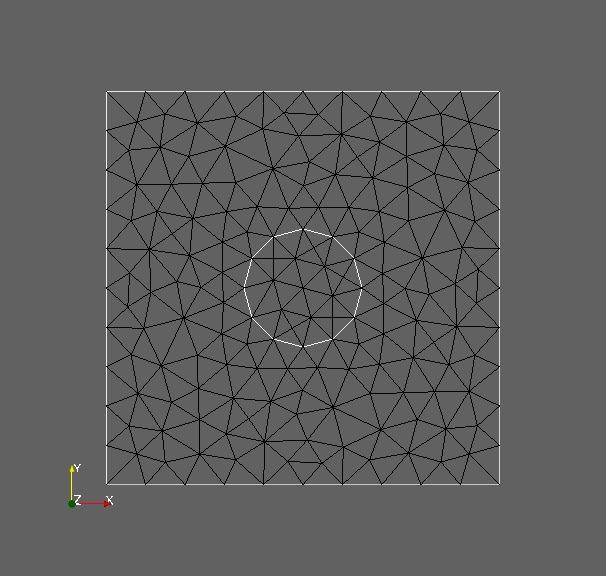
\includegraphics[scale=0.25]{pic_smallcircle.jpg}
	\caption{}	
	\end{subfigure}
	\begin{subfigure}{0.5\textwidth}
	\centering
	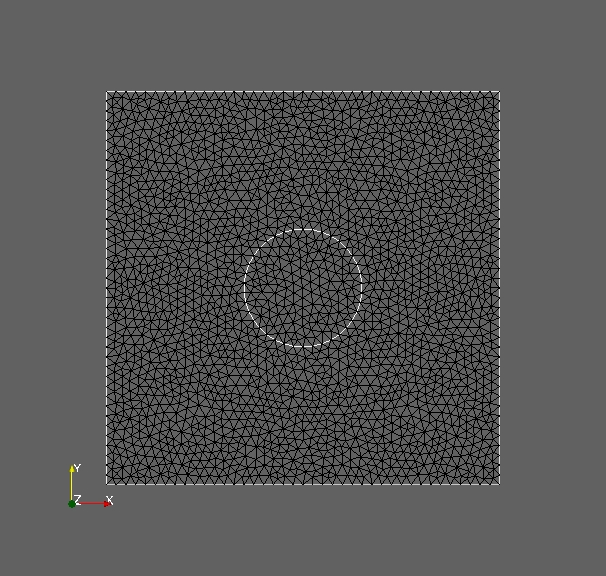
\includegraphics[scale=0.25]{pic_smallcircle_fine.jpg}
	\caption{}	
	\end{subfigure}
	\begin{subfigure}{0.5\textwidth}
	\centering
	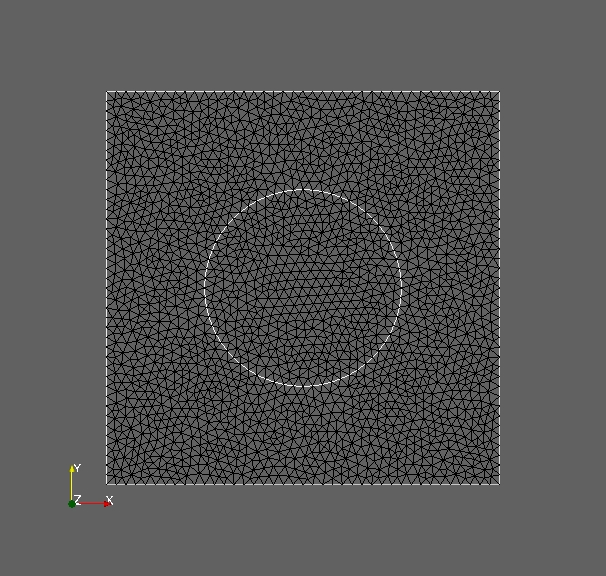
\includegraphics[scale=0.25]{pic_bigcircle_fine.jpg}
	\caption{}	
	\end{subfigure}
	\begin{subfigure}{0.5\textwidth}
	\centering
	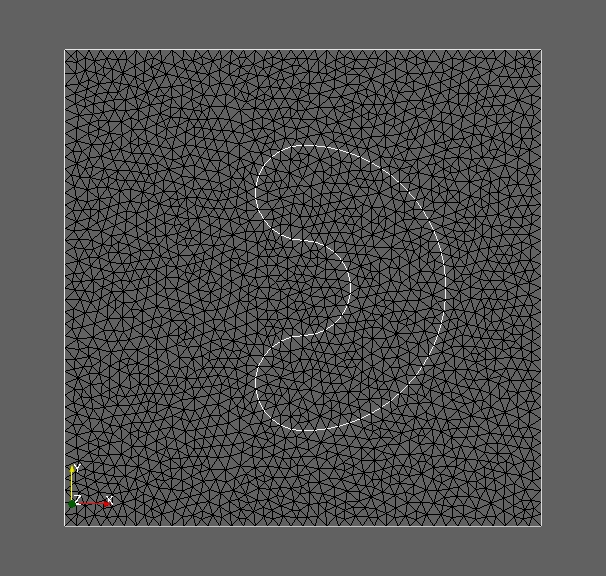
\includegraphics[scale=0.25]{pic_brokendonut_fine.jpg}
	\caption{}	
	\end{subfigure}
\caption{(a) Ausgangsform kleiner Kreis auf grobem Gitter (b) Ausgangsform kleiner Kreis auf feinem Gitter (c) Zielform großer Kreis auf feinem Gitter (d) Zielform broken Donut auf feinem Gitter}
\label{Meshes}
\end{figure}

Wir werden sowohl das L-BFGS-Verfahren, als auch das Gradientenverfahren vergleichen. Außerdem wird jeweils die Linesearch an- und ausgeschaltet, sowie alle oben aufgeführten Parameter, bis auf die Funktionswerte die Zustandsgleichung im Zielgitter, den Verbesserungsfaktor \textsf{c}, und den Skalierungsfaktor \textsf{shrinkage} der Backtracking-Linesearch, variiert. Die Verwendung der Memory-Length von 60 bewirkt, dass es sich in allen folgenden Fällen der Verwendung des L-BFGS-Verfahrens eigentlich um ein BFGS-Verfahren handelt, da die gesamte Historie zur Berechnung der Hesseapproximation benutzt wird. 


Für das Problem der Deformation zum großen Kreis erhalten wir bei dem groben Gitter 
bei Verwendung des Gradientenverfahrens ohne Linesearch Konvergenz nach fast 800 Schritten. Schaltet man das Backtracking ein, so erhält man ebenfalls Konvergenz, jedoch schon bei ca. 450 Schritten. Dies legt nahe, das die Schrittweite durch das anfangliche Hochskalieren der Deformation optimaler wird, der Gradient also der Norm nach relativ klein war. Bei Verfeinerung des Gitters um das 4-fache erhalten wir ebenfalls ohne Verwendung der Linesearch beim Gradientenverfahren Konvergenz nach ca. 650 Schritten. Wieder findet durch Verwendung des Backtracking eine Beschleunigung zur Konvergenz statt, diesmal nach 520 Schritten. Erhöht man das anfangliche Hochskalieren vom Faktor 5 auf 20, so erhält man im feinen Gitter Konvergenz schon nach 120 Schritten. Die Geschwindigkeit zur Konvergenz hat sich also im Vergleich zum Gradientenverfahren ohne Backtracking also um das 5-fache gesteigert, wobei sich die erzeugten Gitter bei Ausstieg des Verfahrens mit oder ohne Linesearch und Veränderung des Hochskalierungsfaktors nicht unterscheiden. 

\colorbox{red}{Plot: feines gitter; no linesearch; linesearch; highstartscale}

Findet das L-BFGS-Verfahren ohne Linesearch Anwendung, so erhält man auf dem groben Gitter keine Konvergenz. Das Verfahren updatet die BFGS-Memory nach mehreren Verletzungen der Curvature Condition nicht, und deformiert das Gebiet schließlich bei Schritt 26 bis zur Unbrauchbarkeit, was in \ref{Destroyedgradient} zu sehen ist. Man beachte die starke Entartung der kaum sichtbaren Zellen kurz vor der Zerstörung des Gitters, welche man im Zoom gut erkennt.


\begin{figure}
	\begin{subfigure}{0.5\textwidth}
	\centering
	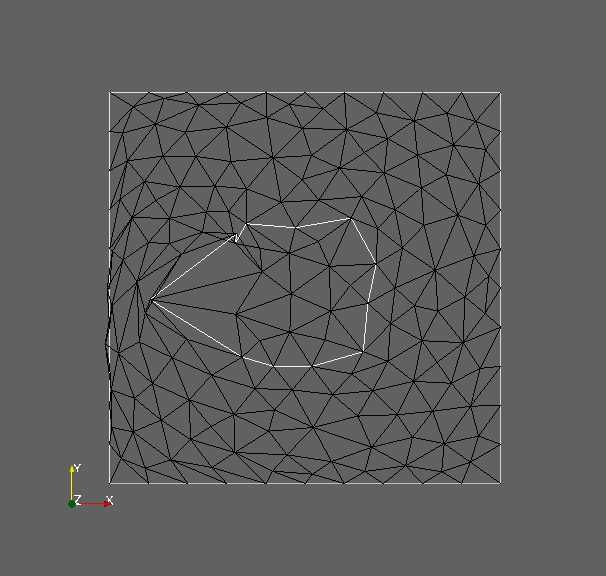
\includegraphics[scale=0.25]{pic_smallcircle_destroyed1.jpg}
	\caption{}	
	\end{subfigure}
	\begin{subfigure}{0.5\textwidth}
	\centering
	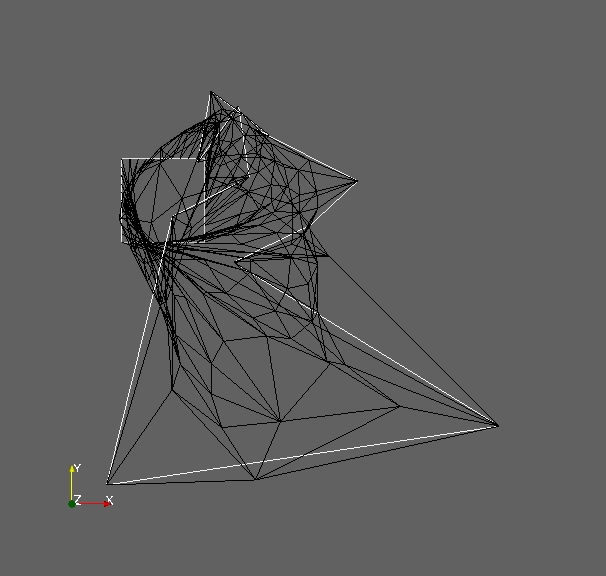
\includegraphics[scale=0.25]{pic_smallcircle_destroyed2.jpg}
	\caption{}	
	\end{subfigure}
\caption{(a) Gitter nach mehrmaligen Schritten unter Verletzung der Curvature Condition und Non-update Schritten (b) der darauf folgende Schritt, Zerstörung des Gitters}
\label{Destroyedgradient}
\end{figure}

Auch bei Verfeinerung des Gitters um das 4-fache erhält man keine Konvergenz des L-BFGS-Verfahrens, sondern erreicht die Zerstörung des Gitters nach Verletzung der Curvature Condition schon im zweiten Schritt, bei der die Form das Einheitsquadrat verlässt. Man beachte, das dieses mal die Richtung des Schrittes in Richtung Optimum geht, jedoch viel zu lang ist, anders als in \ref{Destroyed}, wo zuvor mehrmalige falsche Schritte bei Verletzung der Curvature Condition das Gitter zerstören. Der BFGS-Schritt ist zu sehen in \ref{Destroyedbfgs}. Diese Beobachtung macht erneut deutlich, wie wichtig eine effektive Schrittweitensteuerung bei der Implementierung der Verfahren sind.

\begin{figure}
	\begin{subfigure}{0.5\textwidth}
	\centering
	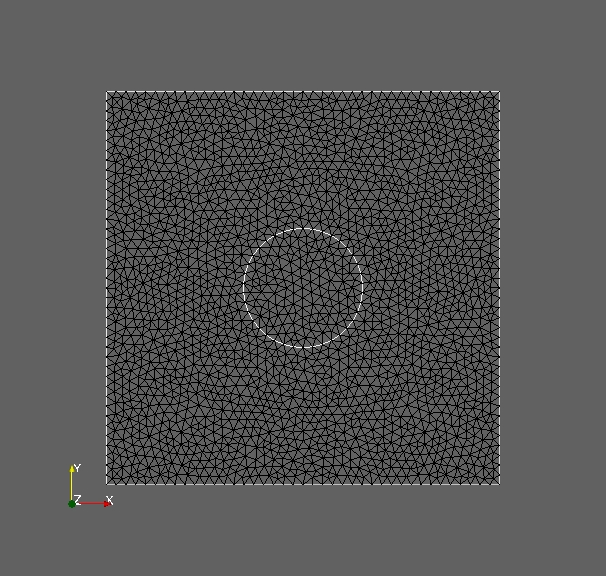
\includegraphics[scale=0.25]{pic_smallcircle_bfgsdestroyed1.jpg}
	\caption{}	
	\end{subfigure}
	\begin{subfigure}{0.5\textwidth}
	\centering
	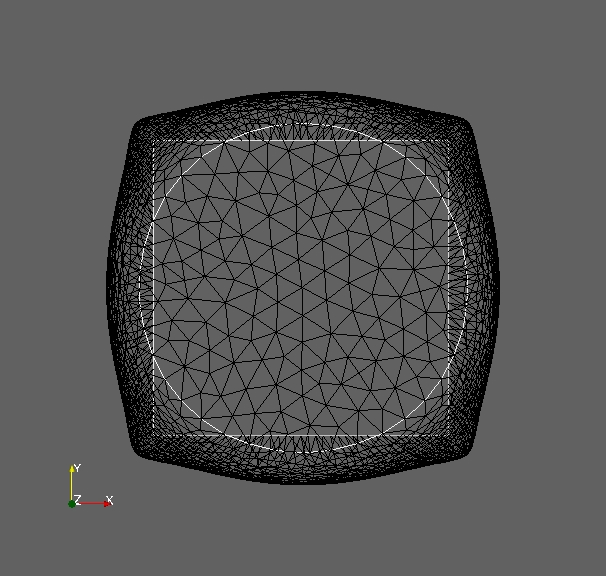
\includegraphics[scale=0.25]{pic_smallcircle_bfgsdestroyed2.jpg}
	\caption{}	
	\end{subfigure}
\caption{(a) 1. Schritt: Gradientenschritt bei feinem Gitter (b) 2. Schritt: BFGS-Schritt mit Entartung des feinen Gitters}
\label{Destroyedbfgs}
\end{figure}

\colorbox{red}{finde raus, warum nur auf der einen Seite kein Text angezeit wird; mache formatierung schöner}

Wir haben auch versucht, die Gitterzerstörung durch Modifikation der lokal variierenden Lamé-Parameter zu begegnen. Alle bisher gezeigten Gitter hatten die Wahl des minimalen Lamé-Parameters von 0. Um zu beobachten, ob die Verfahren instabiler werden, wenn man konstante Lamé-Parameter wählt, haben wir diese konstant auf 30 gesetzt. Man erhält den Output \ref{Destroyedkonstlame}, wobei bei Schritt 5 und 6 die Curvature Condition verletzt sind.

\begin{figure}
	\begin{subfigure}{0.3\textwidth}
	\centering
	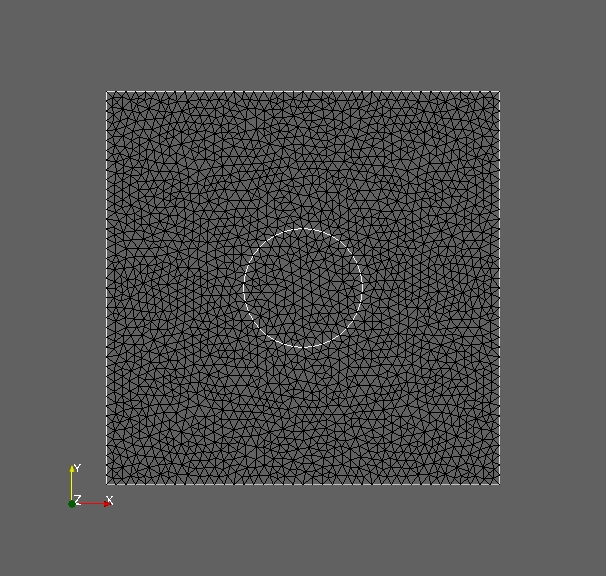
\includegraphics[scale=0.2]{pic_bigcircle_constlame1.jpg}
	\caption{}	
	\centering
	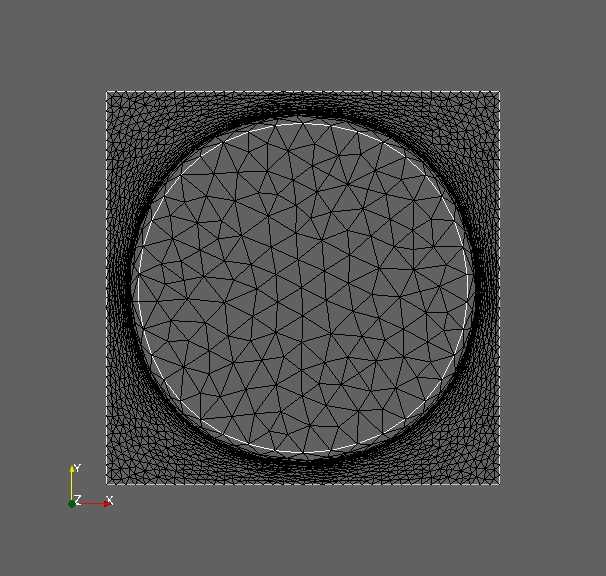
\includegraphics[scale=0.2]{pic_bigcircle_constlame2.jpg}
	\caption{}	
	\end{subfigure}
	\begin{subfigure}{0.3\textwidth}
	\centering
	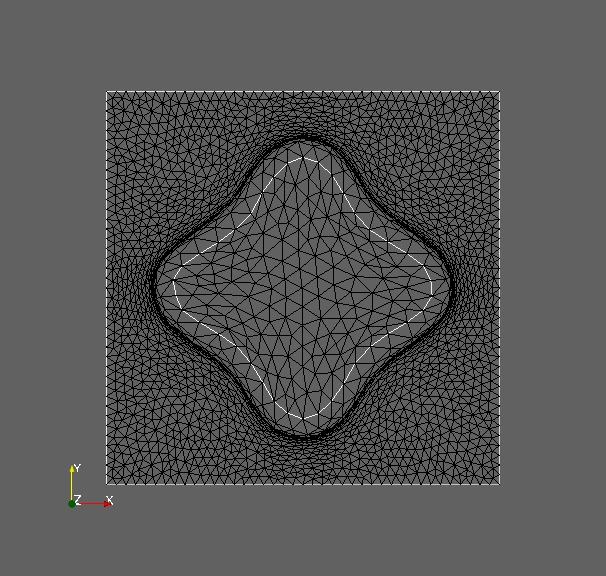
\includegraphics[scale=0.2]{pic_bigcircle_constlame3.jpg}
	\caption{}	
	\centering
	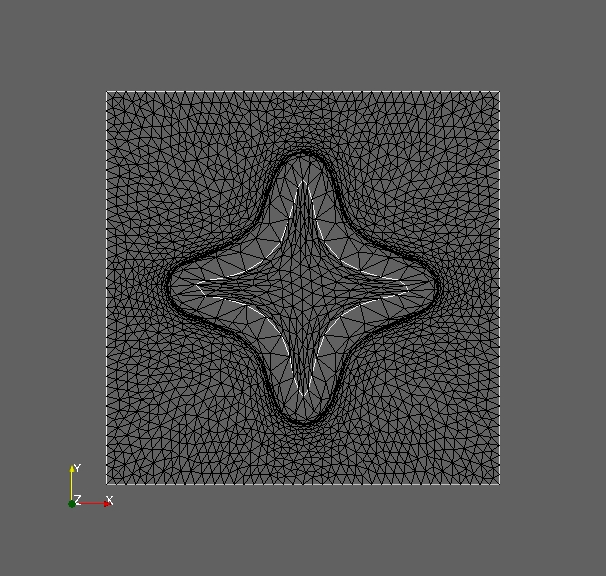
\includegraphics[scale=0.2]{pic_bigcircle_constlame4.jpg}
	\caption{}	
	\end{subfigure}
	\begin{subfigure}{0.3\textwidth}
	\centering
	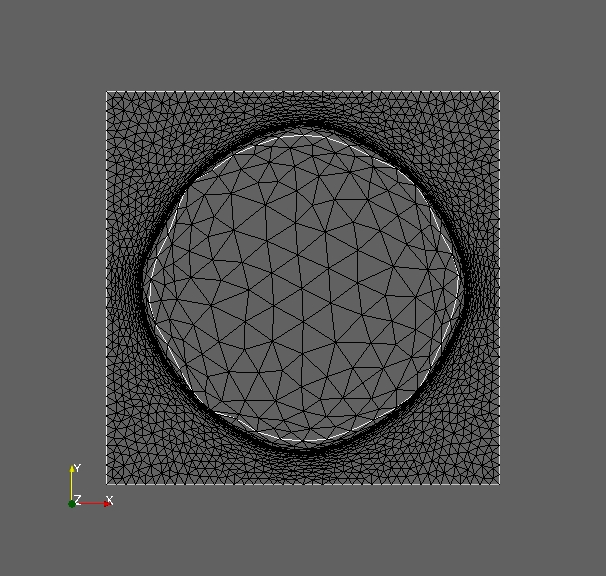
\includegraphics[scale=0.2]{pic_bigcircle_constlame5.jpg}
	\caption{}	
	\centering
	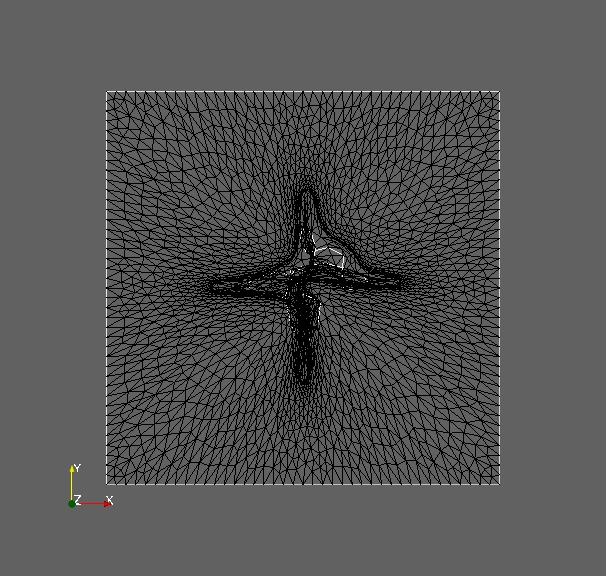
\includegraphics[scale=0.2]{pic_bigcircle_constlame6.jpg}
	\caption{}	
	\end{subfigure}
\caption{BFGS-Verfahren ohne Schrittweitensteuerung bei konstanten Lamé-Parametern mit Wert 30; die ersten 6 Schritte}
\label{Destroyedkonstlame}
\end{figure}

Ein komplett anderes Verhalten stellt sich bei Verwendung der Backtracking-Linesearch ein; in diesem Fall konvergiert das L-BFGS-Verfahren für beide Gitterfeinheiten.
Zudem fällt eine erhebliche Steigerung der Konvergenzgeschwindigkeit auf; schon nach 5 Schritten auf dem groben, und nach 6 auf dem feinen Gitter. 

\colorbox{red}{konvergenzplot der bfgs und gradientenverfahren mit linesearch}

Die bei dem groben Gitter erzeugte optimale Form besitzt noch einen mit bloßem Auge sichtbaren Abstand zur Zielform. In diesem Fall hat unser L-BFGS-Algorithmus bei dem Backtracking maximal herunterskaliert, d.h. keine Abstiegsrichtung gefunden und ist ausgestiegen. Damit scheint ein lokales Minimum erreicht. Bei Verwendung des feinen Gitters ist bei selbem Ausstiegskriterium kein Abstand zur Zielform sichtbar, was man in \ref{Konvergenzbfgscircle} sehen kann.

\begin{figure}
	\begin{subfigure}{0.5\textwidth}
	\centering
	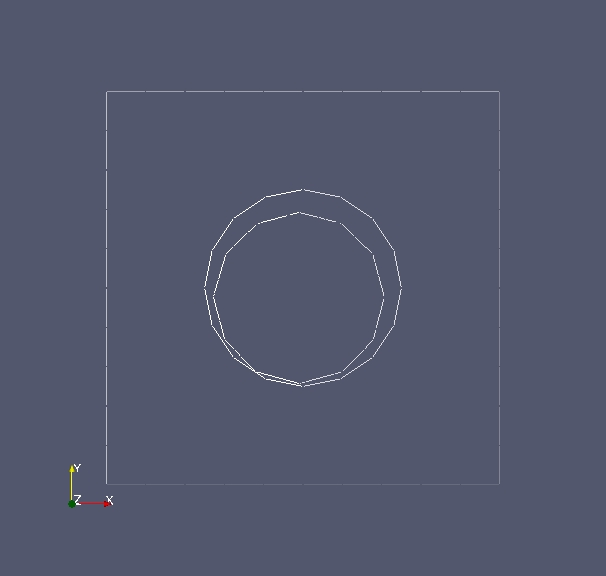
\includegraphics[scale=0.25]{pic_bigcircle_bfgs_linesearch.jpg}
	\caption{}	
	\end{subfigure}
	\begin{subfigure}{0.5\textwidth}
	\centering
	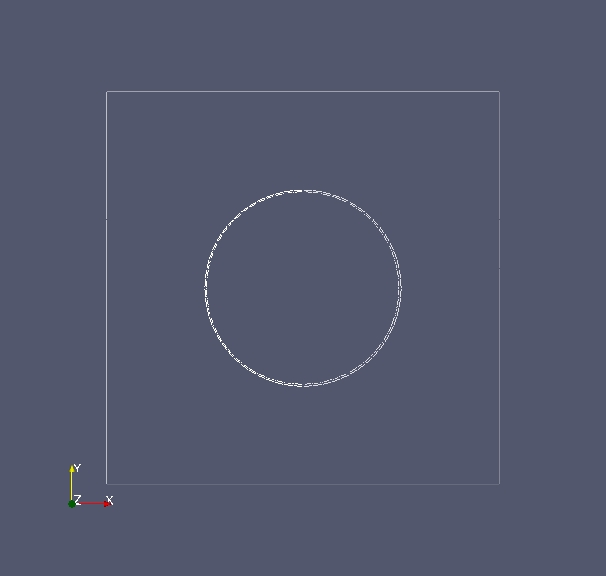
\includegraphics[scale=0.25]{pic_bigcircle_bfgs_linesearch_fine.jpg}
	\caption{}	
	\end{subfigure}
\caption{(a) L-BFGS mit Backtracking bei grobem Gitter. Abweichung bei Ausstieg sichtbar. (b) L-BFGS mit Backtracking bei feinem Gitter. Abweichung bei Ausstieg nicht erkennbar.}
\label{Konvergenzbfgscircle}
\end{figure}

Wir haben durch Veränderung der Perimeter-Regularisierung untersucht, ob sich durch diese der Abstand zur Zielform erklären lässt. Die Vermutung ist, dass die optimale Form etwas kleiner als die Zielform ist, da die Perimeter-Regularisierung kleinere Formen favorisiert. Die in diesem Fall entstehende optimale Lösung ist in diesem Fall symmetrisch mit gleichem Mittelpunkt wie die Zielform, jedoch besitzt sie fast den selben Abstand wie die optimale Form mit der Perimeterregularisierung. Für die Bilder verweisen wir auf die mitgelieferten Dateien auf der CD.

Kontrollieren wir im Falle des BFGS-Algorithmus auf Veränderung bei Erhöhung des Hochskalierungsfaktors \textsf{starscale} des Backtracking, so stellen wir fest, dass die ersten Schritte stärkere Verbesserungen bringen, sobald sich jedoch eine gewisse Memorygröße, und damit eine Hesseapproximation, aufgebaut haben verschwinden diese Effekte wieder, siehe \colorbox{red}{plot beider Graphen; mit linesearch; fine; high und normal startscale}. Dieses Verhalten sollte auftreten, da \colorbox{blue}{BFGS-Schritte mit aufgebauter Hesseapproximation unabhängig einer Skalierung sind}.

Zudem haben wir einen Vergleich zwischen der vollen BFGS-Methode, welche wir durch die \textsf{memory\_length} von 60 erzeugen, und der echten L-BFGS-Methode, mit \textsf{memory\_length} von 2 und 3, im Falle des feinen Gitters gezogen. Interessanterweise stellt sich hier kein merklicher Unterschied hinsichtlich Konvergenzgeschwindigkeit in, was man in \colorbox{red}{plot ref} erkennen kann. Dies lässt sich nach unserer Vermutung dadurch erklären, dass für einen korrekten BFGS-Schritt ein Term \colorbox{red}{ welcher Ordnung?} fehlt. Würde dieser ergänzt, so vermuten wir eine Verbesserung des Algorithmus bei höherer \textit{memory\_length}. Außerdem lässt sich in den Diagrammen keine superlineare Konvergenz nachweisen, welche sich bei korrektem Update möglicherweise einstellt.

\colorbox{red}{hier plot; 3 L-BFGS Memlengths im Zielfunktional}

Neben der bloßen Bedingung einer Verbesserung im Zielfunktional bei dem Backtracking besteht die Möglichkeit, die Amijo-Bedingung für die Linesearch zu verwenden. Diese haben wir nach \cite{Nocedal} implementiert. Verwendet man diese, so konvergiert die L-BFGS-Method nicht mehr, in einigen Fällen konvergiert das Gradientenverfahren. Jedoch würde wir eher behaupten, dass dies \textit{trotz} der Armijo-Bedingung konvergiert. Da diese Bedingung die Verbesserung mit Hilfe eines linearen Modells in der aktuellen Form betrachtet, wäre ein aus der Formoptimierung legitimes anderes Modell vorstellbar, um verbesserte Bedingungen zur Linesearch zu erzeugen. Hierzu hat uns leider die Zeit gefehlt, wir möchten an dieser Stelle jedoch die Relevanz eines solchen Resultats betonen. 

Bei der Berechnung des Formgradienten in \colorbox{red}{referenz implementierung zeroed} haben wir ein Verfahren verwendet, welches in der linearen Elastizitätsgleichung die Punkte, welche nicht Träger des inneren Randes sind, auf Null gesetzt wurden. Schaltet man diese Nullsetzung aus, was durch die Wahl des Parameters \textsf{zeroed = False} möglich ist, so zerstört dies das Verfahren. Sowohl das L-BFGS, als auch das Gradientenverfahren divergieren in allen von uns getesteten Beispielen. Somit tritt des selbe Effekt wie in \cite{bfgs2}, welcher dort in Abschnitt 5, Fig. 2 zu sehen ist. Würde dieser Effekt durch ein Rundungsrauschen hervorgerufen sein, so vermuten wir, dass dieses weniger drastisch sichtbar würde. Bei uns ist schon nach den ersten Schritten das Gitter bis zur Unbrauchbarkeit entartet.

\colorbox{red}{jetzt Donut}

Wir haben die oben genannten Beobachtungen auch für das schwierigere Problem der nierenförmigen, nicht konvexen Form gesammelt. Die Ausgangsform, welcher den kleinen Kreis in \ref{Meshes} darstellt, bleibt gleich, wir wechseln also nur die Zielform, die auch in \ref{Meshes} zu sehen ist. 


\colorbox{red}{zeige nicht alles in Vollem Detail; Bilder zu Konvergenz; Konvergenzplots}

\colorbox{red}{Ausblick und Danksagung an Volker}

Anders als bei dem einfacheren ersten Problem, erhalten wir für ein Gradientenverfahren ohne Backtracking-Linesearch, in den Fällen sowohl des groben, als auch des feinen Gitters, nach ca. 1200, respektive ca. 600 Schritten zwar Konvergenz, jedoch nicht zum globalen Optimum des Zielgitters. Wir vermuten, dass es sich hierbei um lokale Minima handelt, die resultierende optimale Form bleibt konvex, trotz des nicht konvexen Zielgitters, siehe Abbildung
\ref{brokendonutgradient}.

\begin{figure}
	\begin{subfigure}{0.5\textwidth}
	\centering
	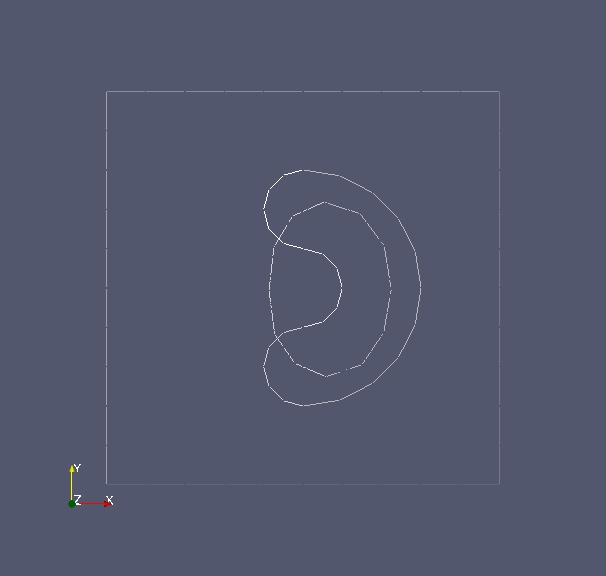
\includegraphics[scale=0.25]{pic_brokendonut_gradient.jpg}
	\caption{}	
	\end{subfigure}
	\begin{subfigure}{0.5\textwidth}
	\centering
	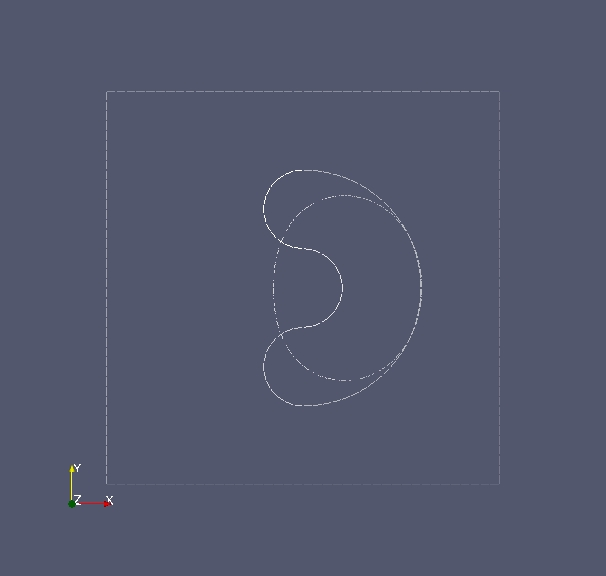
\includegraphics[scale=0.25]{pic_brokendonut_gradient_fine.jpg}
	\caption{}	
	\end{subfigure}
\caption{(a) Optimale Form und Zielform bei Gradientenverfahren auf grobem Gitter (b) Selbiges auf feinem Gitter}
\label{brokendonutgradient}
\end{figure}

Durch das Verwenden der Backtracking-Linesearch schafft es der Algorithmus näher an das globale Optimum zu gelangen. Dies gelingt jedoch ausschließlich bei dem feinen Gitter. Im Falle des groben Gitters erreichen wir auch mit Linesearch die selbe nicht konvexe Form, siehe Abbildung \ref{brokendonutgradient_linesearch}, wobei eine leichte Verbesserung zu sehen ist. Dies zeigt, dass das Verfahren stark abhängig ist von der Gitterfeinheit. \colorbox{red}{frag volker dazu, ob das invariant sein sollte. eigentlich nicht mit hesseinformation oder? oder bilinearform als rim metrik falsche ordnung?}

Außerdem beobachten wir für das Gradientenverfahren, wie im ersten Problem, eine Skalieren der Konvergenzgeschwindigkeit durch das Hochskalieren der Suchrichtung bei dem Backtracking-Linesearch. Wir sparen uns an dieser Stelle die erneute Angabe eines zu \colorbox{red}{plot von skalierung bei erstem Problem} ähnlichen Graphen.
Zudem haben wir in diesem Problem die gleichen Feststellungen bei Verwendung der Armijo-Bedingung bei der Linesearch gemacht, wie bei dem ersten Problem zuvor.

\begin{figure}
	\begin{subfigure}{0.5\textwidth}
	\centering
	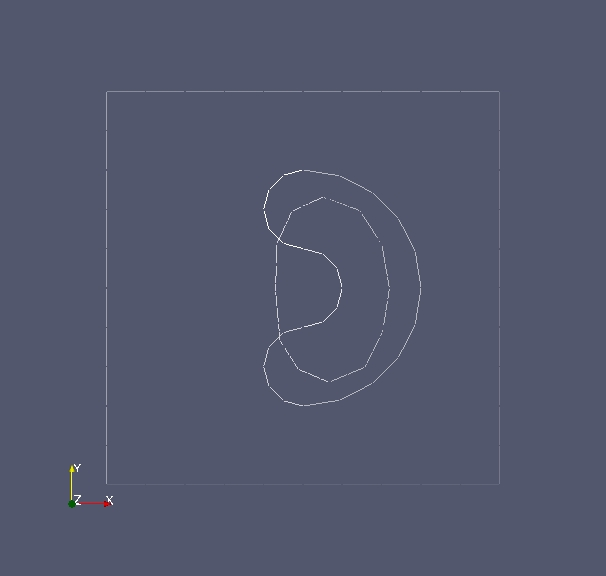
\includegraphics[scale=0.25]{pic_brokendonut_gradient_linesearch.jpg}
	\caption{}	
	\end{subfigure}
	\begin{subfigure}{0.5\textwidth}
	\centering
	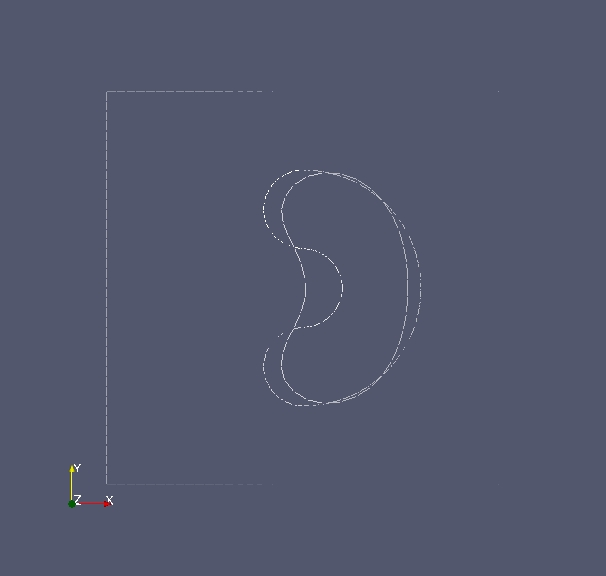
\includegraphics[scale=0.25]{pic_brokendonut_gradient_linesearch_fine.jpg}
	\caption{}	
	\end{subfigure}
\caption{(a) Optimale Form und Zielform bei Gradientenverfahren mit Linesearch auf grobem Gitter (b) Selbiges auf feinem Gitter}
\label{brokendonutgradient_linesearch}
\end{figure}

\colorbox{red}{jetzt bfgs}

Bei Verwendung des L-BFGS-Verfahrens ohne Linesearch bemerken wir, ähnlich wie zu dem ersten Beispiel, dass sowohl beim groben, als auch beim feinen Gitter eine zu \ref{Destroyedbfgs} ähnliche Divergenz stattfindet, weshalb wir uns Graphiken hierzu sparen. Das Gitter ist nach nur wenigen Schritten, nachdem die Curvature Condition verletzt wurde, bis zur Unkenntlichkeit verformt, wobei das Verfahren auch nicht die lokalen Minima \ref{brokendonutgradient_linesearch} oder \ref{brokendonutgradient} erreicht. 

Interessanterweise verbessert sich das Verhalten des L-BFGS-Verfahrens ohne Linesearch, wenn man statt lokal variierenden Lamé-Parametern konstante Lamé-Parameter mit Wert 30 wählt. Zuvor divergierte das Verfahren bei dem feinen Gitter nach nur 5 Schritten unter Verletzung der Curvature Condition der letzten 3 Schritte. Bei konstanten Lamé-Parametern findet zwar auch Divergenz statt, jedoch erst nach 14 Schritten, wobei zuvor sogar ein optimales Ergebniss, welches dem Gradientenverfahren mit Linesearch auf dem feinen Gitter nahe kommt. Zu sehen sind ausgewählte Schritte in \ref{brokendonut_bfgs_konstlame}. Man beachte jedoch den Vergleich zu dem Gitter, welches bei dem L-BFGS-Verfahren mit Linesearch und variierenden Lamé-Parametern erzeugt wird, bei dem geringere Entartung der Zellen des Gitters zu beobachten sind. Wir würden an dieser Stelle vorschlagen, ein Kriterium für die Entartung des Gitters, etwa dem Quotienten aus maximalem und minimalem Zellvolumen, zu verwenden, um bei Überschreitung eines festgelegten Entartungsgrades ein neues Gitter mit der aktuellen Form zu initialisieren. Dies ließe sich auch mit lokal variierenden Lamé-Parametern, sowie mit adaptiven Gittermethoden, kombinieren.

\begin{figure}
	\begin{subfigure}{0.3\textwidth}
	\centering
	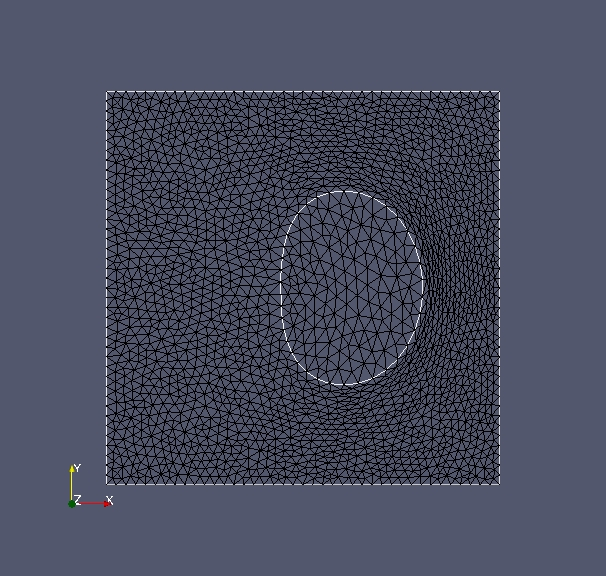
\includegraphics[scale=0.2]{pic_brokendonut_bfgs_konstlame_6.jpg}
	\caption{}	
	\end{subfigure}
	\begin{subfigure}{0.3\textwidth}
	\centering
	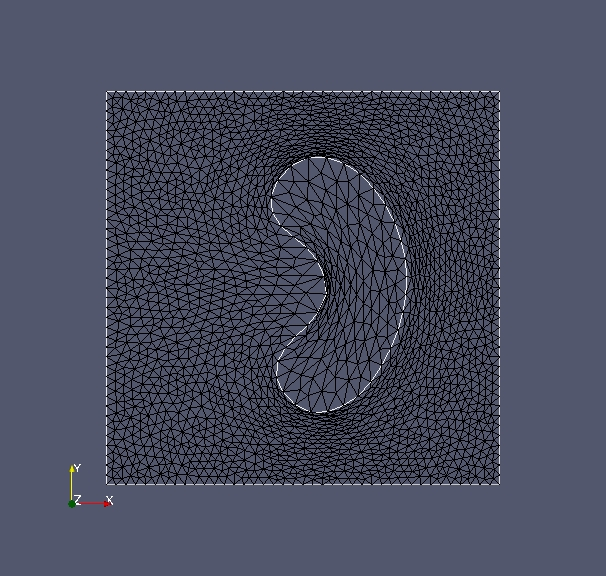
\includegraphics[scale=0.2]{pic_brokendonut_bfgs_konstlame_12.jpg}
	\caption{}	
	\end{subfigure}
	\begin{subfigure}{0.3\textwidth}
	\centering
	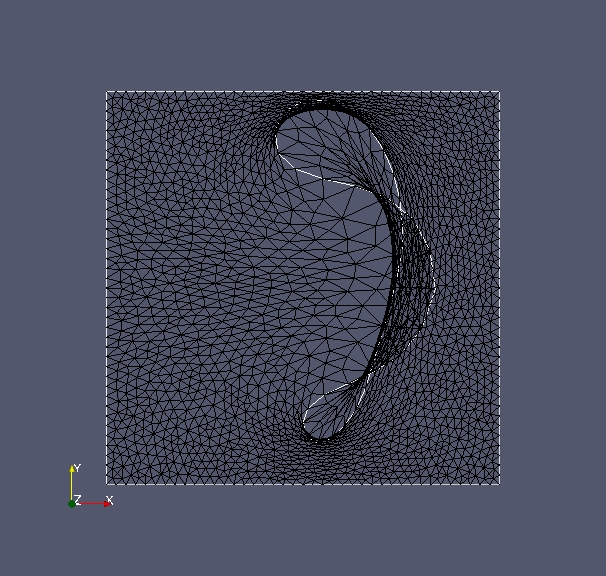
\includegraphics[scale=0.2]{pic_brokendonut_bfgs_konstlame_14.jpg}
	\caption{}	
	\end{subfigure}
\caption{BFGS-Verfahren bei konstanten Lamé-Parameter von 30 (a) Schritt 6 (b) gute Form bei Schritt 12; man beachte die starke Stauchung/ Streckung der Zellen (c) Zerstörung des Gitters bei Schritt 14}
\label{brokendonut_bfgs_konstlame}
\end{figure}

Verwendet man zusammen mit dem L-BFGS-Verfahren die Backtracking-Linesearch, so erhalten wir ähnliche Ergebnisse wie in dem ersten Problem. Eine deutliche Erhöhung der Konvergenzgeschwindigkeit, von ca. 900 Schritten des Gradientenverfahrens mit Linesearch und Startskalierung 5, auf 26 Schritte im Falle des L-BFGS mit Linesearch, auf dem feinen Gitter. Auch auf dem groben Gitter ist eine erhebliche Erhöhung der Konvergenzgeschwindigkeit zu beobachten, wobei auch hier lediglich das lokale Minimum des Gradientenverfahrens erreicht wird. Auf dem feinen Gitter wird, ähnlich dem Gradientenverfahren mit Linesearch, eine sehr gute Lösung erreicht, nahe des globalen Optimums. Damit scheint keine Gitterunabhängigke Konvergenz vorzuliegen. \colorbox{red}{Bilder ref, falls diese verschieden von denen des gradientenverfahrens oben sind, ansonsten auf diese Referenzieren} \colorbox{red}{hat das mit der Ordnung des Hessian zu tun?}
\colorbox{red}{checke, ob konvergenz bei ausstieg, wenn curv. cond. nicht erfüllt ist, auch vorliegt.}
Die Curvature Condition wird ab Schritt 17 verletzt, wobei schon in diesem Schritt eine fast vom Ergebniss kaum zu unterscheidene Lösung erzeugt wird. Die Ausstiegsbedingung war lediglich zu stark gewählt.
Weiterhin stellen wir fest, dass durch das Weglassen der Perimeter-Regularisierung die Konvergenz im \colorbox{red}{perimeter zero vergleich; mit und ohne linesearch}
erhalten bleibt. Lässt man zusätzlich die Lamé-Paramter nicht lokal variieren, so bleibt auch hier die Konvergenz erhalten, das Verfahren benötigt jedoch interessanterweise etwas mehr als die doppelte Anzahl an Schritten. Somit scheint in gewissen Fällen die lokal variierende Wahl der Lamé-Parameter die Konvergenzgeschwindigkeit zu erhöhen. Dieser Effekt tritt bei uns nur in Kombination mit dem Weglassen der Perimeter-Regularisierung auf, wobei in allen Fällen ohne Linesearch Divergenz vorliegt.

Außerdem beobachten wir, dass bei einer Memory-Length von 3, sprich bei einem echte Limited-Memory Ansatz, die Anzahl der benötigten Schritte zur Konvergenz von 26 auf 35 auf dem feinen Gitter, und bei dem groben Gitter gleich bleibt. 
\colorbox{red}{was ist die zugehörige Interpretation?} 
\colorbox{red}{bleibt der Graph ähnlich? wenn ja auf den ersten verweisen}

\begin{figure}
	\begin{subfigure}{0.5\textwidth}
	\centering
	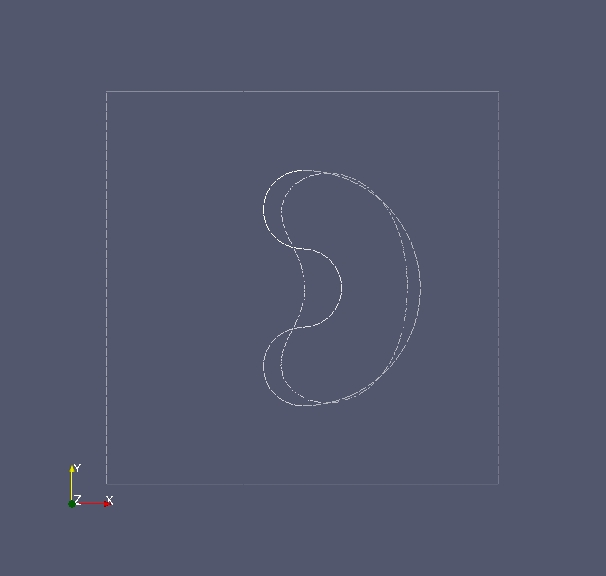
\includegraphics[scale=0.25]{pic_brokendonut_bfgs_linesearch.jpg}
	\caption{}	
	\end{subfigure}
	\begin{subfigure}{0.5\textwidth}
	\centering
	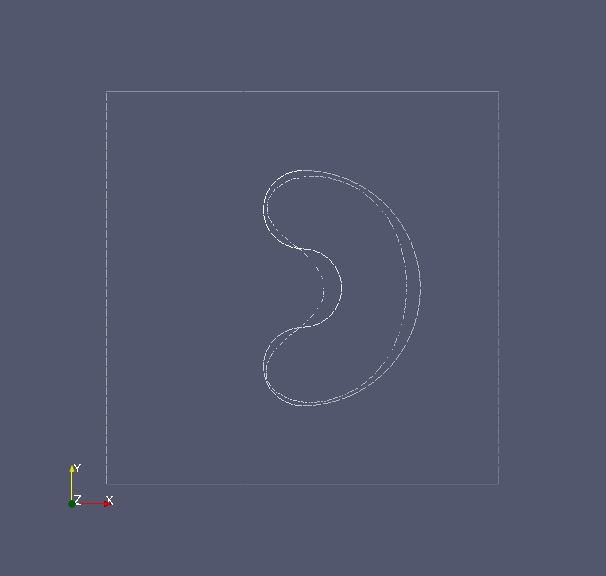
\includegraphics[scale=0.25]{pic_brokendonut_bfgs_linesearch_fine.jpg}
	\caption{}	
	\end{subfigure}
\caption{L-BFGS-Verfahren mit Linesearch (a) Form bei Ausstieg auf grobem Gitter (b) Form bei Ausstieg auf feinem Gitter}
\label{brokendonut_bfgs_linesearch}
\end{figure}

Vergleich mit mem lengths

\colorbox{red}{konvergenzplot von gradient und bfgs bei linesearch}

\colorbox{red}{plot von bfgs und gradienten im vergleich bei linesearch; Kommentar, das bei guter Linesearch vllt beide Verfahren kompetitiv? boosting des Gradienten; erwähne sequential sqp oder wie das heißt (für globable optima)}


\newpage
\nocite{*}
\bibliographystyle{plain}
\bibliography{papers}

\end{document}
